\begin{figure}[t]
\centering
% src: fig/abc_locres_cumulative.png by scripts/paper_figures_abc.py (render --paper); values: docs/paper/fig_abc_locres.csv (window centers with mask >= 0.5)
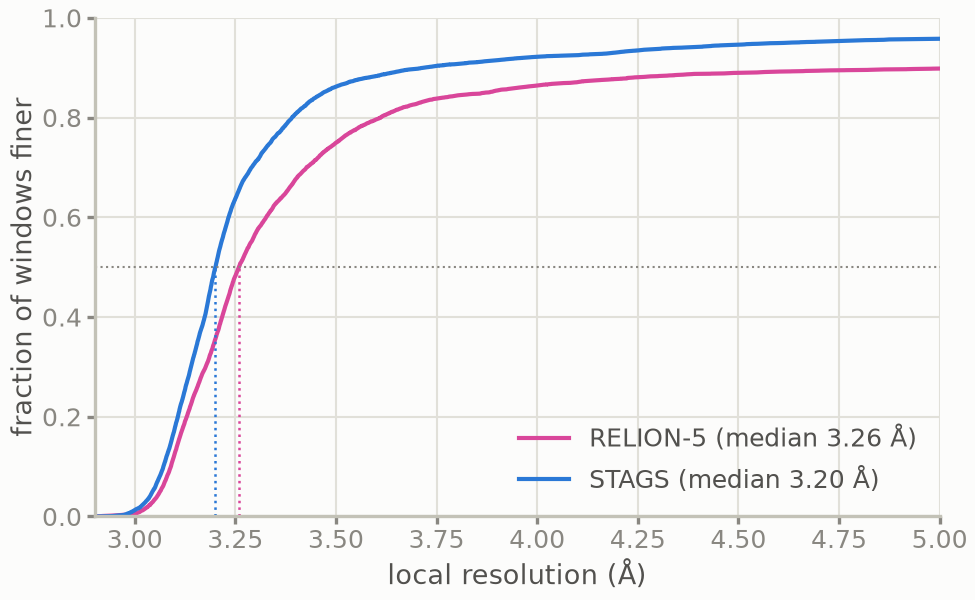
\includegraphics[width=\columnwidth]{fig/abc_locres_cumulative.png}
\caption{\textbf{Distribution of local resolution.}
For each map, the fraction of window centers inside RELION's mask whose local resolution is finer than a given value, from the same estimator as \cref{fig:locres}.
Each median is where its curve crosses one half.
The curves stay below 1 at 5\,\AA\ because some windows, mostly at the mask edge, are coarser.}
\label{fig:locres_cumulative}
\end{figure}
